\section{Brantley--Larsen}
\label{sec:bl}

\subsection{Problem and runs}

One energy group: fuel $\Sigma_t = 1.5$, $\Sigma_{s0} = 1.35$,
$\nu\Sigma_f = 0.24$~cm$^{-1}$; moderator $\Sigma_t = 1.0$,
$\Sigma_{s0} = 0.93$~cm$^{-1}$ (paper Table~5). The fuel bars occupy
$x \in [1,2] \cup [4,5] \cup [7,8]$, $y \in [0,9]$~cm. Every interface lies on
a cell face for $n$ a multiple of 10, so the finite-volume scheme is second
order. Each method was run with Marshak and Robin vacuum on
$n \times n$ meshes, $n = 40, 80, 160, 320, 640$. The GMRES runs of SDP2
(Marshak) and SDP3 (both boundaries) at $n = 640$ would have taken 8--20~h
each on the shared node and were stopped; for those three the extrapolation
uses $n = 80, 160, 320$.

\subsection{Mesh convergence}

\begin{figure}[h]
\centering
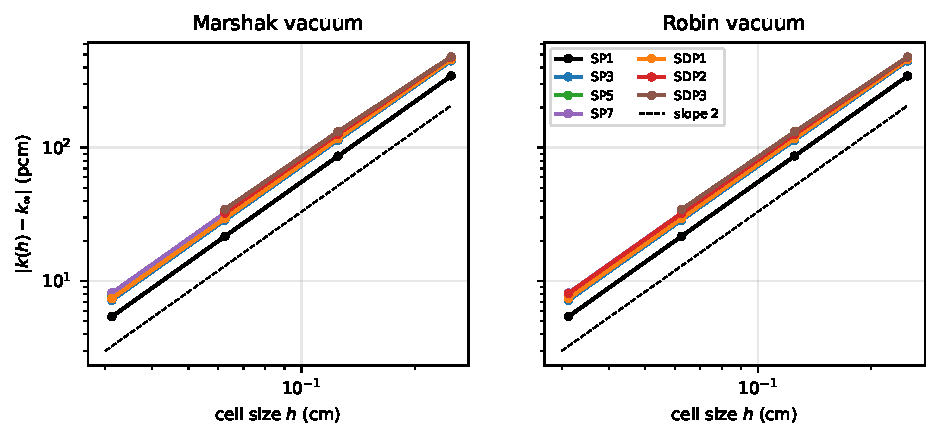
\includegraphics[width=0.82\textwidth]{bl_convergence.pdf}
\caption{Brantley--Larsen: distance of each mesh's $k$ from its own
extrapolated limit. Every method and boundary treatment converges at second
order.}
\label{fig:bl-conv}
\end{figure}

Table~\ref{tab:bl-conv} and Fig.~\ref{fig:bl-conv}. The observed order from
the finest three meshes is between 1.93 and 2.00 for every method and both
vacuum treatments, and $k$ decreases monotonically under refinement.
$k_\infty$ is the Richardson extrapolation with the observed order. The GCI
column is Roache's grid-convergence index with safety factor 1.25; it is
1.7--2.6~pcm where $n = 640$ exists and 10--11~pcm where the triple ends at
$n = 320$. The GCI is a conservative bound: wherever both triples exist
(14 configurations), extrapolating from $n = 80, 160, 320$ and from
$n = 160, 320, 640$ agrees within 0.21~pcm.

\begin{table}[h]
\caption{Brantley--Larsen eigenvalues by mesh, observed order $p$, extrapolated
$k_\infty$ and GCI.}
\label{tab:bl-conv}
\tablefile{bl_convergence}
\end{table}

On the $80 \times 80$ mesh of \path{tests/validation/test_brantley_larsen_2d.py}
the mesh error is $+87$~pcm for SP1 and $+114$ to $+132$~pcm for the
transport methods (Table~\ref{tab:bl-split}). That is larger than the
difference between consecutive SP$_N$ orders above SP5, so single-mesh
comparisons with the paper on that mesh mostly measure mesh error.

\subsection{Comparison with the paper}

\begin{table}[h]
\caption{Brantley--Larsen: extrapolated \garnet{} eigenvalues against the
paper's Table~6 and OpenMOC (pcm). ``Robin $-$ paper'' uses \garnet's
Robin-vacuum $k_\infty$.}
\label{tab:bl-paper}
\tablefile{bl_vs_paper}
\end{table}

\begin{figure}[h]
\centering
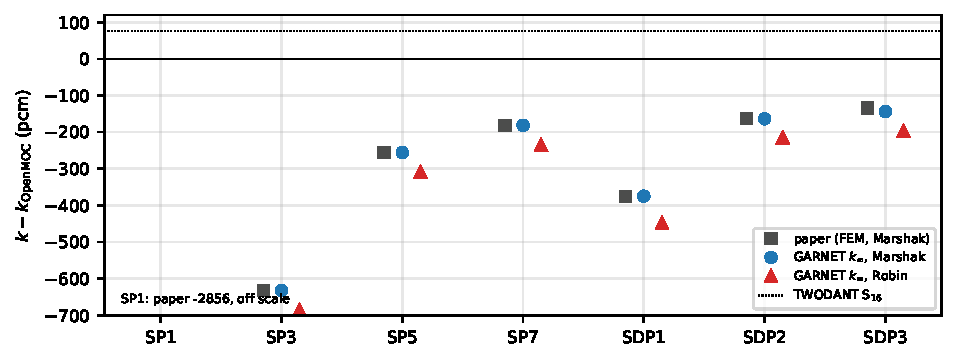
\includegraphics[width=0.82\textwidth]{bl_keff.pdf}
\caption{Brantley--Larsen eigenvalues relative to OpenMOC: paper (finite
elements, Marshak), \garnet{} mesh limit with Marshak and with Robin vacuum.
TWODANT S$_{16}$ is the dotted line.}
\label{fig:bl-k}
\end{figure}

With the Marshak boundary, \garnet's mesh limit equals the paper's Table~6
within 0.6~pcm for SP1, SP3, SP5, SP7, SDP1 and SDP2
(Table~\ref{tab:bl-paper}, Fig.~\ref{fig:bl-k}), about the $\pm 0.5$~pcm
rounding of Table~6. This is the code
verification: the same equations, discretized independently (finite volumes
here, second-degree finite elements in the paper), give the same eigenvalue.

SDP3 is $-9.9$~pcm from the paper. \garnet{} does not use the SDP3
coefficient rows 2--3 printed in the paper's Eq.~(A.6): a from-scratch
symbolic derivation from the paper's own closure reproduces its SDP1 and SDP2
tables and every Marshak matrix exactly, but not those rows
(\path{tests/verification/test_sdpn_derivation.py}, note in
\code{garnet/spn.py}). Section~\ref{sec:a6} shows that the paper's SDP3
values come from a third set, the tables in the authors' FEMFFUSION code,
and that with those \garnet{} reproduces them too.

The Robin vacuum lowers $k$ by 52--54~pcm for every method except SDP1
($-73$~pcm). It was the default of every solver except the dedicated SP3
when this study started; Marshak is now the default wherever it is available,
and Robin is kept for comparison.

The angular error, $k_\infty - k_{\rm OpenMOC}$ with Marshak, is
$-2856$~pcm for diffusion, $-632$, $-256$ and $-181$~pcm for SP3, SP5, SP7,
and $-375$, $-163$ and $-144$~pcm for SDP1, SDP2, SDP3. At equal numbers of
moments SDP$_N$ is closer to transport than SP$_{2N+1}$ (SDP1/SP3,
SDP2/SP5, SDP3/SP7), the paper's central claim, and it holds with the
re-derived SDP3 tables. The two transport references differ by 77~pcm
(TWODANT S$_{16}$ above OpenMOC), which is about half the remaining SDP3 and
SP7 errors: the references do not resolve which of those two is closer to
transport.

\subsection{Error budget on the test mesh}

\begin{table}[h]
\caption{Brantley--Larsen error budget (pcm). Mesh error is $k_{80} - k_\infty$
with Marshak. The last two columns are the single-mesh comparison of the
validation test on the $80 \times 80$ mesh, with each vacuum treatment.}
\label{tab:bl-split}
\tablefile{bl_split}
\end{table}

Table~\ref{tab:bl-split} splits the single-mesh comparison into its parts.
With Marshak, every method is $+87$ to $+127$~pcm above the paper on the
$80 \times 80$ mesh, and all of it is mesh error (for SDP3, less the
$-10$~pcm of its re-derived tables). With Robin the offset is
smaller, $+45$ to $+73$~pcm, only because two errors of opposite sign add:
mesh error and the Robin offset ($-52$ to $-73$~pcm). Under the old Robin
defaults the test's 150~pcm envelope therefore passed partly by
cancellation; it now checks the Marshak results, and the Robin offset
separately.

\subsection{Equivalent code paths}

\begin{table}[h]
\caption{Dedicated solvers against the general SP$_N$/SDP$_N$ block of the same order.}
\label{tab:bl-eq}
\tablefile{bl_equivalence}
\end{table}

SP3 and SDP1 each have a dedicated two-moment solver and can also be run
through the general block of order 1 (Table~\ref{tab:bl-eq}). With Marshak,
the dedicated SP3 solver and the SP$_N$ block agree to $2 \times 10^{-10}$ on
every mesh: two independent implementations of the coupled boundary. With
Robin they differ by up to 0.7~pcm (SP3) and 0.35~pcm (SDP1), because the
dedicated solvers apply $\alpha = 1/2$ to $(\Phi_1, \phi_2)$ and the general
block to its $U$ moments. The per-moment Robin term is an approximation
whose result depends on the choice of moments; the Marshak condition is not.

\subsection{Flux along $y = 4.5$~cm}

\begin{figure}[h]
\centering
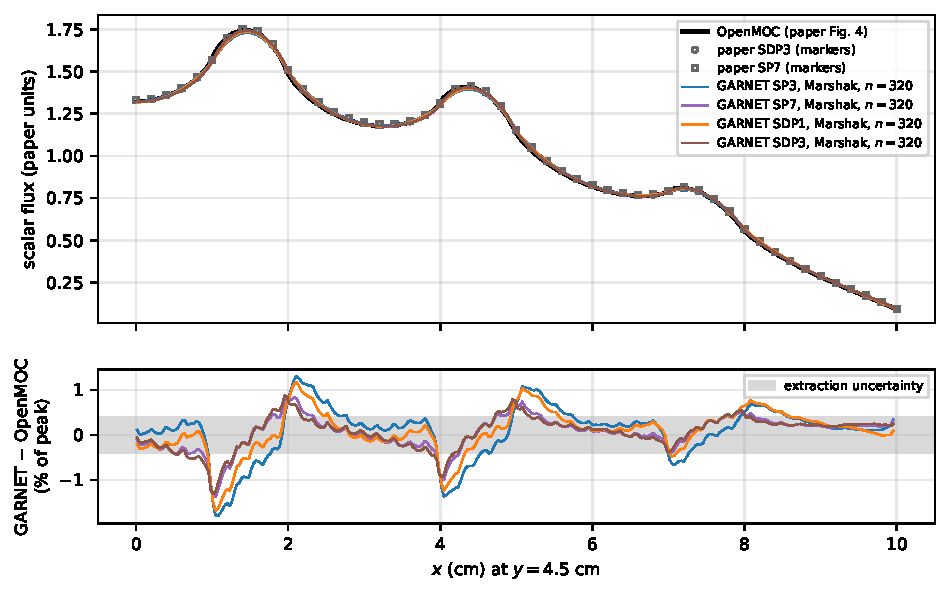
\includegraphics[width=0.85\textwidth]{bl_flux_line.pdf}
\caption{Scalar flux along $y = 4.5$~cm: OpenMOC and the paper's SDP3 and SP7
markers (paper Fig.~4) and \garnet{} with Marshak vacuum. \garnet{} curves are
scaled to OpenMOC by least squares. Lower panel: \garnet{} minus OpenMOC; the
grey band is the extraction uncertainty.}
\label{fig:bl-flux}
\end{figure}

\begin{table}[h]
\caption{Flux along $y = 4.5$~cm against OpenMOC, after a least-squares scale
(\% of the OpenMOC peak).}
\label{tab:bl-flux}
\tablefile{bl_flux}
\end{table}

Fig.~\ref{fig:bl-flux} and Table~\ref{tab:bl-flux}. \garnet's SDP3 and SP7
deviate from OpenMOC by 0.36--0.37\% of the peak (RMS), the paper's own SDP3
and SP7 markers by 0.39--0.40\%. Both are at the extraction uncertainty
(0.39\%), so on this line the two codes agree with transport equally well.
The remaining structure, up to 1.8\% of the peak, sits at the fuel-bar edges,
where the angular flux is most anisotropic; SP3 is the largest there and SDP3
the smallest. The paper's markers, 0.2~cm apart, are too sparse to show it.

\subsection{The paper's printed SDP3 tables}
\label{sec:a6}

Three sets of SDP3 coefficient tables are in circulation, and they differ only
in the closure rows 2--3:

\begin{itemize}
\item \textbf{Re-derived} (\garnet's default): rows 2--3 obtained symbolically
  from the paper's own closure, Eq.~(34). The same derivation reproduces the
  paper's SDP1 and SDP2 tables and all three Marshak matrices exactly.
\item \textbf{FEMFFUSION}: the tables in the authors' code
  (\path{src/matrix_operators/matrix_operators_sdpn.cc}).
\item \textbf{Paper (A.6)}: the tables as printed. They equal FEMFFUSION's
  except row 2 of $c^{(3)}$, printed as $(36/55,\ 54/175)$ where the code has
  $(9/25,\ -54/175)$.
\end{itemize}

\begin{table}[h]
\caption{Brantley--Larsen SDP3 with Marshak vacuum and the three coefficient
sets. $k_\infty$ is extrapolated from $n = 80, 160, 320$.}
\label{tab:bl-a6}
\tablefile{bl_sdp3_tables}
\end{table}

On Brantley--Larsen (Table~\ref{tab:bl-a6}) the FEMFFUSION tables give a
mesh limit 0.2~pcm from the paper's 0.80402, the re-derived tables
$-9.9$~pcm and the printed tables $+23.6$~pcm. The paper's SDP3 results were
therefore computed with the FEMFFUSION tables, and with them \garnet{}
reproduces Table~6 for all seven methods. On C5G7 at $s = 4$ the FEMFFUSION
tables raise SDP3 by 14.3~pcm and the printed ones by 15.2~pcm.

Which tables are right is a question of derivation, which this benchmark
cannot settle. The re-derived rows are the only ones of the three that follow
from the closure the paper states, and
\path{tests/verification/test_sdpn_derivation.py} keeps them in place. The
choice moves $k$ by 10--15~pcm on these problems, small against SDP3's
angular error ($-144$~pcm against OpenMOC on Brantley--Larsen).



\subsection{Cost}

\begin{table}[h]
\caption{Brantley--Larsen cost at $n = 160$, best of three solves on one CPU
thread (merlin7 \code{cn000}). Inner iterations are operator applies of the
within-group Krylov solver. The paper's CPU times are for its own $80 \times 80$
finite-element mesh and are listed only for scale.}
\label{tab:bl-cost}
\tablefile{bl_cost}
\end{table}

Table~\ref{tab:bl-cost}. At $n = 160$ (25\,600 cells, one group) the SP$_N$
solves take 0.8--3.8~s with nearly the same inner work for every order
(3088--3357 operator applies): the cost grows with the size of the block,
not with the number of iterations, and the Marshak boundary costs SP$_N$
nothing measurable (CG either way). SDP1 and SDP2 with Robin vacuum are
symmetrized and solved by CG at about the cost of SP3 and SP5. With Marshak
their block is non-symmetric and runs GMRES: 1.5 times the applies but 5--6
times the time (8.0 and 13.0~s), the rest being GMRES's orthogonalization.
SDP3 has no symmetric form once a vacuum face is present and runs GMRES with
either boundary (18--19~s). The paper's CPU times refer to its own mesh and
machine and are listed for scale only.

